\documentclass{beamer}
\usepackage{notation}
\usepackage{forloop}
\usepackage{hyperref}

\usepackage{mathtools}  
\mathtoolsset{showonlyrefs}  
% \usepackage[dvipsnames]{xcolor}

\usetheme{metropolis}           % Use metropolis theme
\title{Gaussian Processes}
\date{\today}
\author{Nipun Batra}
\institute{IIT Gandhinagar}
% \hypersetup{colorlinks=true,linkcolor=magenta,filecolor=magenta,urlcolor=magenta,
% 	linkbordercolor=magenta,
% pdfborderstyle={/S/U/W 1}
% }
\begin{document}
	\maketitle
	
	
	
	\section{Gaussian Distribution}
	\begin{frame}{1D Gaussian Scatter Plot}
		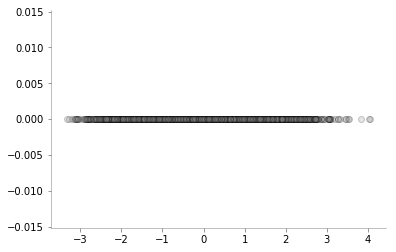
\includegraphics[width=\linewidth,height=\textheight,keepaspectratio]{gp/1d-gp}
	\end{frame}
	
	\begin{frame}{1D Gaussian Histogram}
		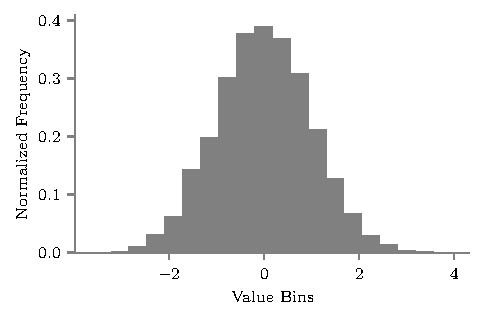
\includegraphics[width=\linewidth,height=\textheight,keepaspectratio]{gp/1d-gp-hist}
	\end{frame}
	
	\begin{frame}{Varying 1D Gaussian Variance}
		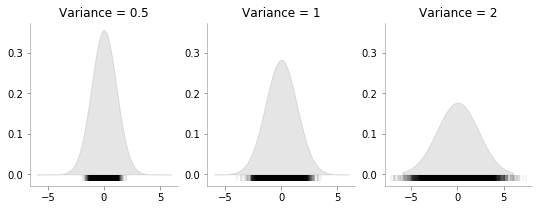
\includegraphics[width=\linewidth,height=\textheight,keepaspectratio]{gp/1d-gp-kde2}\end{frame}
	
	\begin{frame}{Bi-variate Gaussian}
		$$
		\begin{pmatrix}
		X_1 \\
		X_2
		\end{pmatrix}  \sim \mathcal{N} \left( \begin{pmatrix}
		\mu_1 \\
		\mu_2
		\end{pmatrix} , \begin{pmatrix}
		a &\rho \\
		\rho & b
		\end{pmatrix} \right)
		$$\\
		
		\begin{center}
			$\rho$ denotes the correlation between $X_1$ and $X_2$.
			
			$b$ denotes the variance of $X_1$.
			
			$a$ denotes the variance of $X_2$.
		\end{center}
		
	\end{frame}
	
	\begin{frame}{Sampling Bi-variate Gaussian - 1}
		\begin{center}
			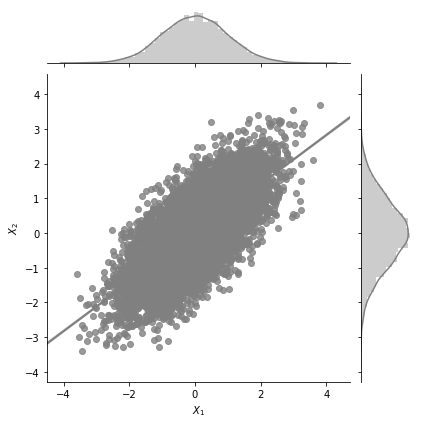
\includegraphics[height=\textheight -45pt ,keepaspectratio]{gp/2d-gp}\\
			Here the covariance between the two random variables is positive.
		\end{center}
	\end{frame}
	
	
	\begin{frame}{Sampling Bi-variate Gaussian - 2}
		\begin{center}
			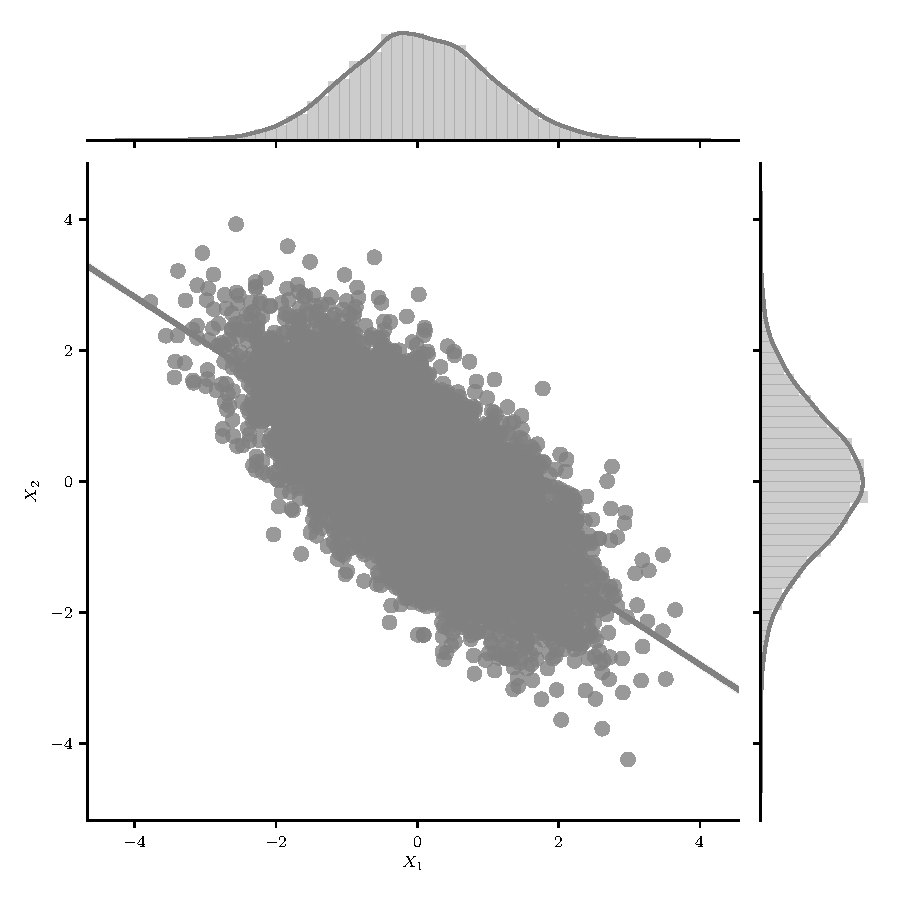
\includegraphics[height=\textheight -45pt ,keepaspectratio]{gp/2d-gp2}\\
			Here the covariance between the two random variables is negative.
		\end{center}
	\end{frame}
	
	\begin{frame}{Sampling Bi-variate Gaussian - 3}
		\begin{center}
			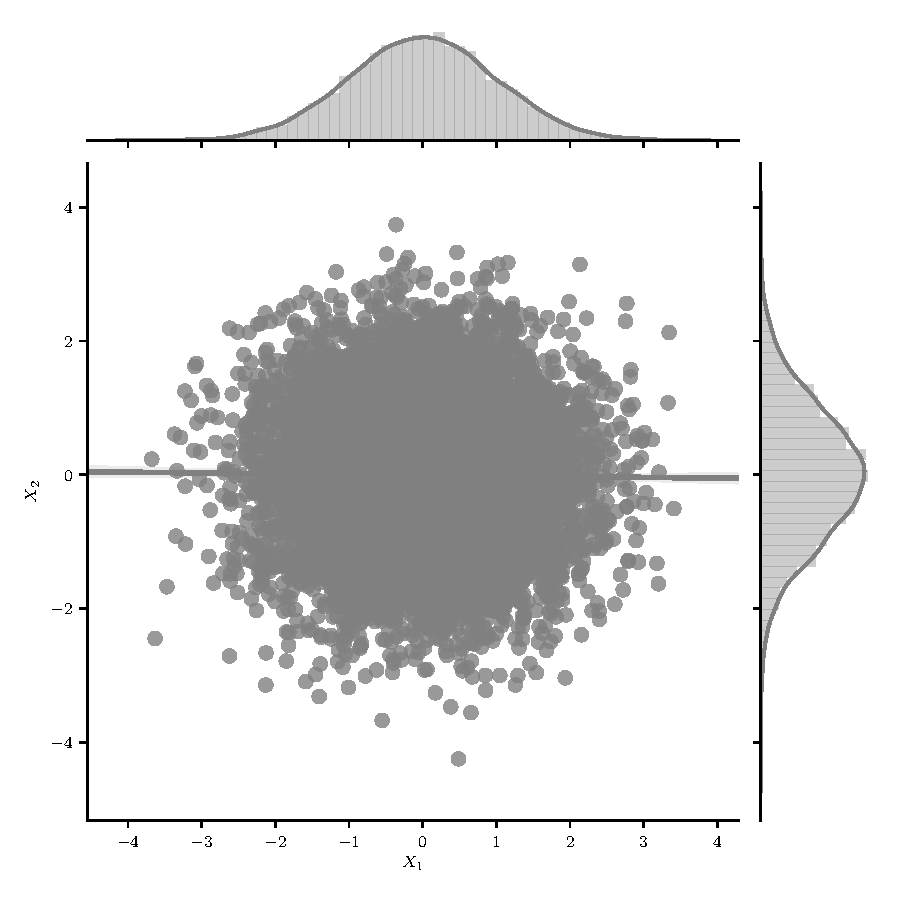
\includegraphics[height=\textheight -30pt ,keepaspectratio]{gp/2d-gp3}\\
			The two random variables are uncorrelated.
		\end{center}
	\end{frame}
	
	\begin{frame}{Surface Plots Bi-variate Gaussian - 1}
		\begin{center}
			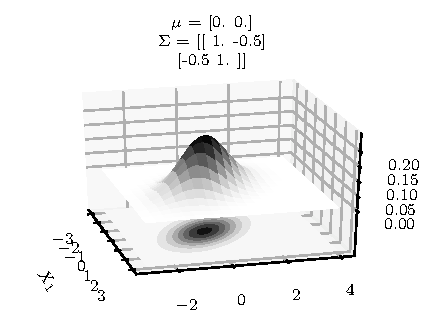
\includegraphics[height=\textheight -10pt ,keepaspectratio]{gp/2dgp3d}
		\end{center}
	\end{frame}
	
	\begin{frame}{Surface Plots Sampling Bi-variate Gaussian - 2}
		\begin{center}
			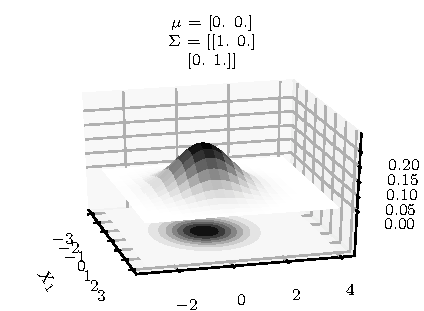
\includegraphics[height=\textheight -10pt ,keepaspectratio]{gp/2dgp3d2}
		\end{center}
	\end{frame}
	
	\section{Visualizing samples from 2D Gaussian}
	
	% for cov
	\newcounter{iter}
	\forloop{iter}{1}{\value{iter} < 6}%
	{%
		\begin{frame}{Cov = 0.1 | Random State - \theiter}
			\includegraphics[width=\linewidth,height=\textheight,keepaspectratio]{gp/0.1/\theiter}\\
			One can notice, increasing the $\rho$ (or the covariance) between $X_1$ and $X_2$ results in the realizations of $X_1$ and $X_2$ to increasingly move together.
		\end{frame}
	}
	% for cov
	\forloop{iter}{1}{\value{iter} < 6}%
	{%
		\begin{frame}{Cov = 0.7 | Random State - \theiter}
			\includegraphics[width=\linewidth,height=\textheight,keepaspectratio]{gp/0.7/\theiter}\\
			One can notice, increasing the $\rho$ (or the covariance) between $X_1$ and $X_2$ results in the realizations of $X_1$ and $X_2$ to increasingly move together.
		\end{frame}
	}
	
	\section{Conditional Bi-variate Distribution}
	
	\begin{frame}{Conditional Bi-variate Distribution}
		$$
		\begin{pmatrix}
		X_1 \\
		X_2
		\end{pmatrix}  \sim \mathcal{N} \left( \begin{pmatrix}
		0 \\
		0
		\end{pmatrix} , \begin{pmatrix}
		1 & \rho \\
		\rho & 1
		\end{pmatrix} \right)
		$$
		
		The conditional expectation of $X_2$ given $X_1$ is: $\operatorname{E}(X_2 \mid X_1=x_1)= \rho x_1$
		
		and the conditional variance is: $\operatorname{var}(X_2 \mid X_1 = x_1) = 1-\rho^2$
	\end{frame}
	
	% for cov
	\forloop{iter}{1}{\value{iter} < 6}%
	{%
		\begin{frame}{Conditional bi-variate | Cov = 0.1 | Random State - \theiter}
			\includegraphics[width=\linewidth,height=\textheight,keepaspectratio]{gp/conditional/0.1/\theiter}\\
			Notice that upon fixing the first random variable, the variance of the second random variable $X_2$ is a function of the covariance ($\rho$) between the two random variables.
		\end{frame}
	}
	
	% for cov
	\forloop{iter}{1}{\value{iter} < 6}%
	{%
		\begin{frame}{Conditional bi-variate | Cov = 0.7 | Random State - \theiter}
			\includegraphics[width=\linewidth,height=\textheight,keepaspectratio]{gp/conditional/0.7/\theiter}\\
			Notice that upon fixing the first random variable, the variance of the second random variable $X_2$ is a function of the covariance ($\rho$) between the two random variables.
		\end{frame}
	}
	
	\section{5D Multivariate}
	
	% for cov
	\forloop{iter}{1}{\value{iter} < 6}%
	{%
		\begin{frame}{Multivariate Gaussian Sample | Random State - \theiter}
			\begin{center}
				\includegraphics[width=\linewidth, height=\textheight -120pt ,keepaspectratio]{gp/5d/\theiter}
			\end{center}
			From the visualisation above we can see that:
			\begin{itemize}
				\item Since $X_1$ and $X_2$ are highly correlated, they move up and down together
				\item but, $X_1$ and $X_5$ have low correlation, thus, they can seem to wiggle almost independently of each other.
			\end{itemize}
		\end{frame}
	}
	
	\section{Conditional Multivariate Distribution}
	
	%\begin{frame}
	%	The idea that is that we can extend this modelling technique to any number of random variables.
	%\end{frame}
	
	\urldef\urlwik\url{https://en.wikipedia.org/wiki/Multivariate\_normal\_distribution#Conditional\_distributions}
	
	\label{sec:condMul}
	\begin{frame}{Conditional Multivariate Distribution Definition\footnote{\urlwik}}
		If $N$-dimensional $\mathbf{x}$ is partitioned as follows
		$$\mathbf{x}
		=
		\begin{bmatrix}
		\mathbf{x}_A \\
		\mathbf{x}_B
		\end{bmatrix}
		\text{ with sizes }\begin{bmatrix} q \times 1 \\ (N-q) \times 1 \end{bmatrix}$$
		and accordingly $\mathbf{\mu}$ and $\mathbf{\Sigma}$ are partitioned as follows
		$$\boldsymbol\mu
		=
		\begin{bmatrix}
		\boldsymbol\mu_A \\
		\boldsymbol\mu_B
		\end{bmatrix}
		\text{ with sizes }\begin{bmatrix} q \times 1 \\ (N-q) \times 1 \end{bmatrix}$$
		$$\boldsymbol\Sigma
		=
		\begin{bmatrix}
		\boldsymbol\Sigma_{AA} & \boldsymbol\Sigma_{AB} \\
		\boldsymbol\Sigma_{BA} & \boldsymbol\Sigma_{BB}
		\end{bmatrix}
		\text{ with sizes }\begin{bmatrix} q \times q & q \times (N-q) \\ (N-q) \times q & (N-q) \times (N-q) \end{bmatrix}$$	
	\end{frame}
	
	\begin{frame}
		then the distribution of $\mathbf{x}_A$ conditional on $\mathbf{x}_B = \mathbf{b}$ is multivariate normal $(\mathbf{x}_A|\mathbf{x}_B=b)\sim \mathcal{N}(\bar{\mathbf{\mu}}, \bar{\mathbf{\Sigma}})$
		$$\bar{\boldsymbol\mu}
		=
		\boldsymbol\mu_A + \boldsymbol\Sigma_{AB} \boldsymbol\Sigma_{BB}^{-1}
		\left(
		\mathbf{B} - \boldsymbol\mu_B
		\right)$$
		and covariance matrix
		$$\overline{\boldsymbol\Sigma}
		=
		\boldsymbol\Sigma_{AA} - \boldsymbol\Sigma_{AB} \boldsymbol\Sigma_{BB}^{-1} \boldsymbol\Sigma_{BA}.$$
		
	\end{frame}
	
	% for cov
	\forloop{iter}{1}{\value{iter} < 6}%
	{%
		\begin{frame}{Conditional Multivariate Distribution | Random State - \theiter}
			\begin{center}
				\includegraphics[width=\linewidth, height=\textheight -120pt ,keepaspectratio]{gp/5d/conditional/1/\theiter}
			\end{center}
			From the visualisation above we can see that:
			\begin{itemize}
				\item Since the covariance between $X_4$ and $X_5$ is high, $X_4$ moves such that it's value is similar to the fixed value of $X_5$.
				\item Since covariance between $X_1$ and $X_5$ is low, thus the realizations of $X_1$ are uncorrelated to the fixed value of $X_5$.
			\end{itemize}
		\end{frame}
	}
	
	\begin{frame}{20 Dimensional Multivariate}
		\begin{center}
			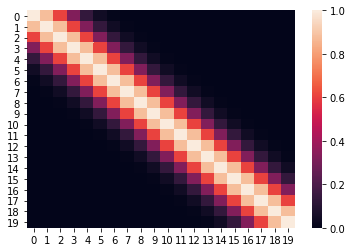
\includegraphics[width=\linewidth, height=\textheight -120pt ,keepaspectratio]{gp/20d}\\
		\end{center}	
		The above heatmap shows that there is high covariance value between nearby points, but close to zero or zero covariance otherwise.
	\end{frame}
	
	% for cov
	\forloop{iter}{1}{\value{iter} < 6}%
	{%
		\begin{frame}{Multivariate (20D) Distribution Samples | Random State - \theiter}
			\begin{center}
				\includegraphics[width=\linewidth, height=\textheight -120pt ,keepaspectratio]{gp/20d/\theiter}
			\end{center}
			From the animation above, we can see different family of functions of mean zero across 20 points. Notice that nearby points are more correlated (making the curve smooth) than the points farther away.
		\end{frame}
	}
	
	\section{Learning from Data}
	
	\begin{frame}{Adding new Data Points}
		Now we want to update the model with new data. We find the functional value at the points $X_1, X_2, X_6, X_{11}$.
		
		We will be using the equations at the start of \hyperref[sec:condMul]{section} Conditional multivariate distribution, to update or Guassian Process, in the wake of new data points.
	\end{frame}
	
	\begin{frame}{Updated Covariance Matrix}
		\begin{center}
			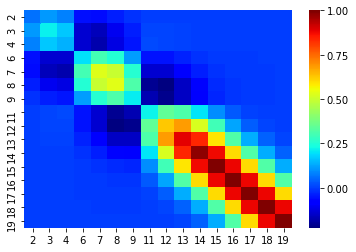
\includegraphics[width=\linewidth, height=\textheight -120pt ,keepaspectratio]{gp/post20d}
		\end{center}
		Notice that the variance of the points near the newly added data points seem to have reduced.
	\end{frame}
	
	% for cov
	\forloop{iter}{1}{\value{iter} < 6}%
	{%
		\begin{frame}{Conditional Multivariate (20D) Distribution Samples | Random State - \theiter}
			\begin{center}
				\includegraphics[width=\linewidth, height=\textheight -120pt ,keepaspectratio]{gp/20d/conditional/\theiter}
			\end{center}
			From the animation above, we can see points near the added data points (red) seem to have a much lower variance compared to points far off.
		\end{frame}
	}
	
	\begin{frame}{Multivariate (20D) Posterior}
		\begin{center}
			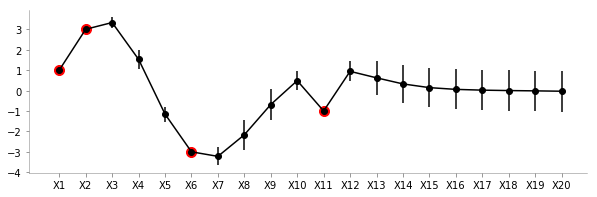
\includegraphics[width=\linewidth, height=\textheight -120pt ,keepaspectratio]{gp/20dcov} \\
		\end{center}
		We can easily see the reduced variance in this plot.
	\end{frame}
	
	\urldef\urlsek\url{http://evelinag.com/Ariadne/covarianceFunctions.html}
	\section{Kernels!}
	\begin{frame}{Defining Squared Exponential Kernel}
		We will now dive a bit into kernels. These are functions that are used to generate the covariance matrix.
		
		Below we have defined, what is known as the Squared Exponential Kernel\footnote{\urlsek}. \\
		
		We have 2 parameters the define this kernel.
		\begin{itemize}
			\item $\sigma$ is the scale of variance.
			\item $l$ is the influence of the point to the neighbouring points
		\end{itemize}
		
		$$
		k(x_1, x_2) = \sigma^2 \exp\left(-\frac{(x_i - x_j)^2}{2l^2}\right)
		$$
	\end{frame}
	
	\begin{frame}{Varying $l$ with $\sigma = 1$}
		\begin{center}
			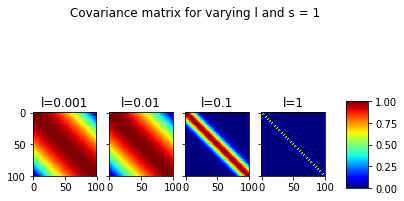
\includegraphics[width=\linewidth, height=\textheight -120pt ,keepaspectratio]{gp/vary_l}\\
			As it can be seen with the plots above, using a smaller $l$ means the function is much more smoother. Using a larger $l$, as in the case when $l = 1$, we see the covariance between two points that are far off, falls to zero.
		\end{center}
		
	\end{frame}
	
	\begin{frame}{Varying $\sigma$ with $l = 0.1$}
		\begin{center}
			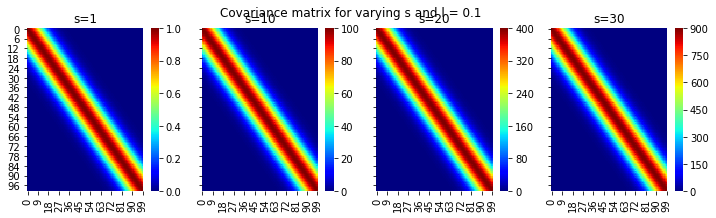
\includegraphics[width=\linewidth, height=\textheight -120pt ,keepaspectratio]{gp/vary_s}\\
			As it can be seen with the plots above, a small $s$ keeps the variance and covariance values small. Whereas, a bigger $s$ leads to higher values of variance and covariance. One thing to notice is that we are talking about covariance, not correlation, $s$ doesn't affect the correlation between random variables.
		\end{center}
	\end{frame}
	
	\begin{frame}{Varying kernel parameters on 20D Guassian with conditioning}
		\begin{center}
			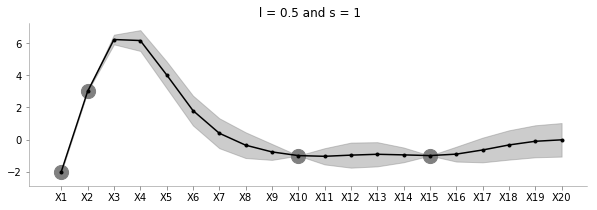
\includegraphics[width=\linewidth, height=\textheight -120pt ,keepaspectratio]{gp/kernel/20gp_ker1}\\
			The big dark circles in the above plot denote the fixed points on which the GP is conditioned. Furthermore, notice the translucent areas, denoting the variance and the smoothness of the function denoting the correlation between random variables.
			
			We have used the squared exponential kernel introduced earlier in this example.
		\end{center}
	\end{frame}
	
	\begin{frame}{Varying kernel parameters on 20D Guassian with conditioning}
		\begin{center}
			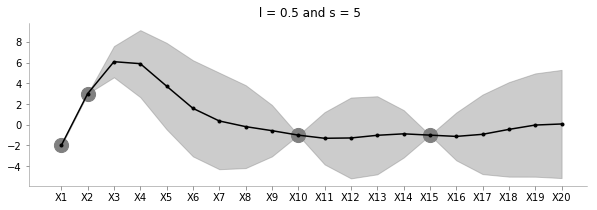
\includegraphics[width=\linewidth, height=\textheight -120pt ,keepaspectratio]{gp/kernel/20gp_ker2}\\
			We can notice the increase in the variance of each of the random variables by increasing the value of $s$ parameter of the kernel.
		\end{center}
	\end{frame}
	
	\begin{frame}{Varying kernel parameters on 20D Guassian with conditioning}
		\begin{center}
			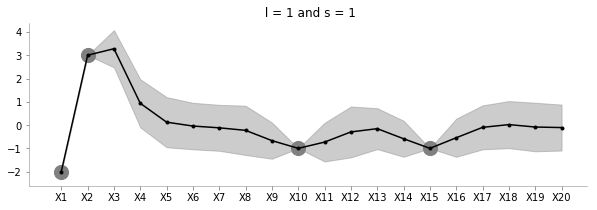
\includegraphics[width=\linewidth, height=\textheight -120pt ,keepaspectratio]{gp/kernel/20gp_ker3}\\
			Increasing the value of $l$ reduces the correlation between nearby points. We, therefore, see that the resulting curve is rougher.
		\end{center}
	\end{frame}
	
	\begin{frame}{Varying kernel parameters on 20D Guassian with conditioning}
		\begin{center}
			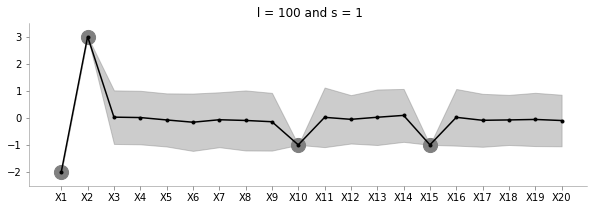
\includegraphics[width=\linewidth, height=\textheight -120pt ,keepaspectratio]{gp/kernel/20gp_ker4}\\
			Keeping a huge value of $l$ results in the conditioned random variables to be highly uncorrelated with the fixed points, as can be seen above. Further, the conditioned points just move around the mean, which is set to zero in this example.
		\end{center}
	\end{frame}
	
	\section{Formalization of Gaussian Processes}
	
	\begin{frame}{Gaussian Processes}
		A Gaussian process is fully specified by a mean function $m(\mathbf{x})$ and covariance function $K(\mathbf{x}, \mathbf{x'})$
		
		$$f(\mathbf{x}) \sim GP (m(\mathbf{x}),K(\mathbf{x}, \mathbf{x'}))$$
		
		where $\mathbf{x}$ is a vector and $f$ is a real-valued function, i.e. $f: {\rm I\!R}^n \rightarrow {\rm I\!R}$.
	\end{frame}
	
	\begin{frame}{Noiseless GPs}
		We will first consider the case of noiseless GPs. This case assumes that for a particular $\mathbf{x}$, we would always receive a single functional value $f(\mathbf{x})$, i.e., there is no inherent noise in our function.
	\end{frame}
	
	\begin{frame}{Noiseless GPs}
		Given train data:
		
		$$D = {(\mathbf{x_i}, y_i), i = 1:N}$$
	\end{frame}
	
	
	\begin{frame}{Noiseless GPs}
		Given a test set $\mathbf{X}_{\ast}$ of size $N_{\ast} \times d$ containing $N_{\ast}$ points in $\mathbf{R}_d$, we want to predict function outputs $y_{\ast}$.
		
		We can write:
		
		$$\begin{pmatrix}
		\mathbf{y} \\
		\mathbf{y}_*
		\end{pmatrix}  \sim \mathcal{N} \left( \begin{pmatrix}
		\bm{\mu} \\
		\bm{\mu}_*
		\end{pmatrix} , \begin{pmatrix}
		\mathbf{K} & \mathbf{K}_* \\
		\mathbf{K}_*^T & \mathbf{K}_{**}
		\end{pmatrix} \right)$$
		
		where:
		
		\begin{gather}
		\mathbf{K} = Ker(\mathbf{X}, \mathbf{X}) \in {\rm I\!R}^{N\times N} \label{eq1}\\
		\mathbf{K}_* = Ker(\mathbf{X}, \mathbf{X}_*) \in {\rm I\!R}^{N\times N_*} \label{eq2}\\
		\mathbf{K}_{**} = Ker(\mathbf{X}_*, \mathbf{X}_*) \in {\rm I\!R}^{N_*\times N_*} \label{eq3}
		\end{gather}
	\end{frame}
	
	\begin{frame}{Noiseless GPs}
		Conditioning Gaussian results into another Gaussian. We get the following mean and covariance matrix postconditioning.
		
		\begin{gather}
		p(\mathbf{y}_*|\mathbf{X}_*, \mathbf{X}, \mathbf{y}) \sim \mathcal{N}(\bm{\mu}', \bm{\Sigma}')
		\end{gather}
		
		where:
		
		\begin{gather}
		\bm{\mu}' = \bm{\mu}_* + \mathbf{K}_*^T\mathbf{K}^{-1}(\mathbf{x}-\bm{\mu}) \\
		\bm{\Sigma}' = \mathbf{K}_{**} - \mathbf{K}_*^T\mathbf{K}^{-1}\mathbf{K}_*
		\end{gather}
	\end{frame}
	
	
	\begin{frame}{GP Updates - Cholesky Decomposition}
		If we notice the last slide, we used a matrix inversion while trying to find the updated covariance matrix. In practical settings, matrix inversions are usually avoided due to multiple reasons. Some of them being:
		
		\begin{enumerate}
			\item Numerically unstable
			\item Computationally heavy
		\end{enumerate}
		
		In some cases where we can avoid matrix inversion, therefore it is preferred to do so.
	\end{frame}
	
	\begin{frame}{GP Updates - Cholesky Decomposition}
		$\mathbf{K}$ is a semi positive definite matrix. Such matrices can be decomposed using cholesky decomposition. Which can be written as:
		
		$$\mathbf{A} = \mathbf{L L}^T$$
		
		where:
		
		$\mathbf{L}$ is a lower triangular matrix with real and positive diagonal entries.	
		
		We can thus re-write the posterior mean and covariance as:
		
		\begin{gather}
			p(y_*|X_*, X, y) \sim \mathcal{N}(\mu', \Sigma') \\
			K = LL^T
		\end{gather}
	\end{frame}

	\begin{frame}{GP Updates - Cholesky Decomposition}
		We are now going to use the \textbackslash \ as follows: if $\mathbf{Aω}=\mathbf{B}$, then $\mathbf{ω} = \mathbf{B} \textbackslash \mathbf{A}$. We now have:
		\begin{gather}
			\alpha = K^{-1}(x-\mu) \\
			\text{or, } \alpha = {LL^T}^{-1}(x-\mu) \\
			\text{or, } \alpha = L^{-T}L^{-1}(x-\mu) \\
			\text{Let, } K^{-1}(x-\mu) = \beta \\
			\text{Thus, } L^{-T}L^{-1}(x-\mu) = \beta \\
			\text{Let, } L^{-1}(x-\mu) = \gamma\\
			\text{Thus, } L\gamma = x-\mu \\
			\text{Thus, } \gamma = L \setminus (x-\mu)\\\
			\text{Thus, } \alpha = L^{T} \setminus (L \setminus (x-\mu))
		\end{gather}
		
		We can therefore have avoid matrix inversion.
	\end{frame}

	
	
\end{document}